\documentclass[../EngineeringJournal_CDavis.tex]{subfiles}

\begin{document}

%%%%%%%%%%%%%%%%%%%%%%%%%%%%%%%%%%%%%%%%%%%%%%%%%%%%%
%%%%%%%%%%%%%%%%%%%%%%%%%%%%%%%%%%%%%%%%%%%%%%%%%%%%%

\chapter[Basic Switch Configuration]{Basic Switch\linebreak[1]
Configuration \hspace*{\fill February 21, 2020}}
\noindent\textbf{{Packet Tracer Lab 09} \hspace*{\fill}{\textbf{CIT 167}}}\linebreak[1]
{{Spring 2020} \hspace*{\fill}{Chaz Davis}}                             
%===================================
%===================================


\hspace{0.2cm}
\begin{tcolorbox}[width=6.3in]
\scriptsize 
switch shit
  \begin{outline}
    \1 something something commands
  \end{outline}
\end{tcolorbox}
\hspace{0.2cm}
\normalsize  

\clearpage

%===================================
\mysection{\textbf{Part 1: Cable the Network and Verify the Default Switch
Configuration}}

\mysubsection{1}{Cable the Network}
I set up the network according to the topography, see
Fig.~\ref{Sconfig9.1}\subref{Sconfig9cable} on Pg.Pg.~\pageref{Sconfig9.1}. I went to the flash memory
on the switch, and there was no vlan.dat configuration. So I proceeded to the
next step. 
\hfill\break

\noindent\mysubsection{2}{Verify the default switch Configuration}

\noindent{\bf{a)}}
I ran the enable command to log into priviledged
exec mode and ran the following commands:
\hfill\break

\noindent{\bf{b)}}
We can see in Fig.~\ref{Sconfig9.1}\subref{Sconfig9runconfig} on
Pg.~\pageref{Sconfig9.1} that the switch has 24 fast ethernet ports
and that the switch has 2 gigabit ethernet ports. We can also see that the
vty lines have the values 0 4 and 5 15.
\hfill\break

\noindent{\bf{c)}}
In Fig.~\ref{Sconfig9.2}\subref{Sconfig9startup} on Pg.~\pageref{Sconfig9.2}
that we do indeed get the 
response {\scriptsize{\verb$startup-config is not present$}\normalsize}, 
this is because we have not configured any settings, and
have in fact reset the switch.
\hfill\break

\noindent{\bf{d)}}
From the output of Fig.~\ref{Sconfig9.2}\subref{Sconfig9intvlan1} on
Pg.~\pageref{Sconfig9.2} that that there is no ip address assigned yet, because
we have not set it up yet, and that the mac address is 00e0.f9bd.263e.
\hfill\break

\noindent{\bf{e and f)}}
You can see in Fig.~\ref{Sconfig9.2}~\subref{Sconfig9intvlanpconnect} 
on Pg.~\pageref{Sconfig9.2} that protocols are down and vlan 1 is not set up yet.
It's showing multicast and fifo settings after hookup.
\hfill\break

\noindent{\bf{g)}}
You can see in Fig.~\ref{Sconfig9.3}~\subref{Sconfig9showver} 
on Pg.~\pageref{Sconfig9.3} that the Cisco IOS version on the switch is
12.2(25)FX, and the system image filename C2960-LANBASE-M, and the mac address
is 00e0.f9bd.263e.
\hfill\break

\noindent{\bf{h)}}
You can see in Fig.~\ref{Sconfig9.3}~\subref{Sconfig9showint6} 
on Pg.~\pageref{Sconfig9.3} that the interface is up because we connected it to
the PC. mac address is 00e0.b037.9co6. The speed of the switch is 100mb/s and
it is full duplex. 
\hfill\break

\noindent{\bf{i)}}
You can see in Fig.~\ref{Sconfig9.3}~\subref{Sconfig9showvlan} 
on Pg.~\pageref{Sconfig9.3} that the name of vlan 1 is default, currently all
ports on on vlan 1, the default type is ethernet.

\begin{figure}[!b]\centering
\subfloat[Cabling the Network]{\label{Sconfig9cable}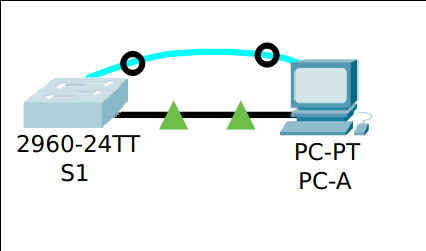
\includegraphics[width=.45\linewidth]{Figures/2020-02-20-125412_426x251_scrot.png}}\hfill
\subfloat[show running config output]{\label{Sconfig9runconfig}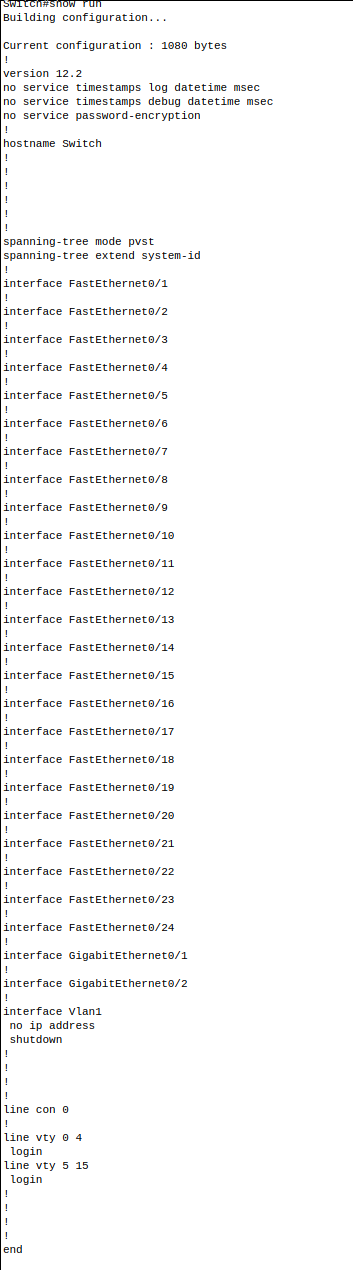
\includegraphics[width=.45\linewidth]{Figures/2020-02-20-125749_353x1270_scrot.png}}\par
\caption{Configuring and verifying the switch Pt 1}
\label{Sconfig9.1}
\end{figure}

\begin{figure}[!b]\centering
\subfloat[show startup config]{\label{Sconfig9startup}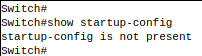
\includegraphics[width=.45\linewidth]{Figures/2020-02-20-125821_202x56_scrot.png}}\hfill
\subfloat[show interface vlan1]{\label{Sconfig9intvlan1}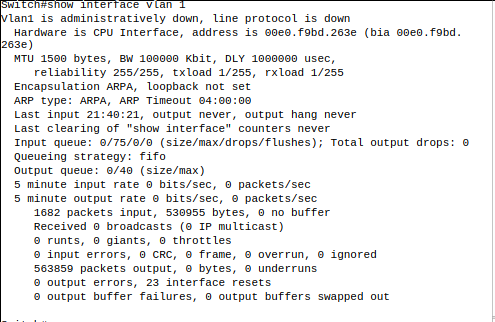
\includegraphics[width=.45\linewidth]{Figures/2020-02-20-125922_495x322_scrot.png}}\par
\hfill\break

\subfloat[show ip interface vlan1 after connecting the ethernet
cable]{\label{Sconfig9intvlanpconnect}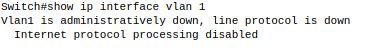
\includegraphics[width=.60\linewidth]{Figures/2020-02-20-130000_373x53_scrot.png}}\par
\caption{Configuring and Verifying the switch Pt 2}
\label{Sconfig9.2}
\end{figure}


\begin{figure}[!b]\centering
\subfloat[show version output]{\label{Sconfig9showver}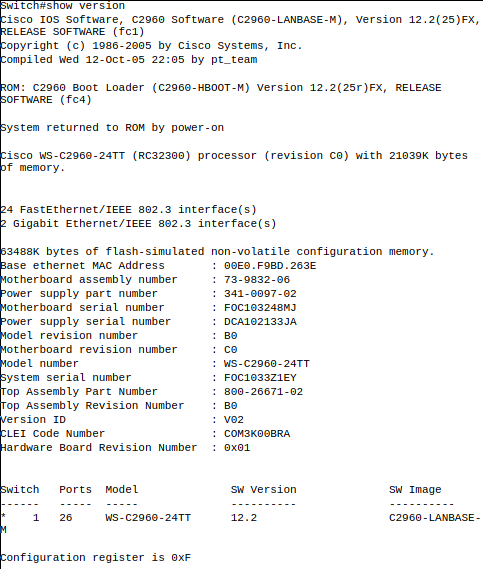
\includegraphics[width=.45\linewidth]{Figures/2020-02-20-130114_483x569_scrot.png}}\hfill
\subfloat[show interface f0/6]{\label{Sconfig9showint6}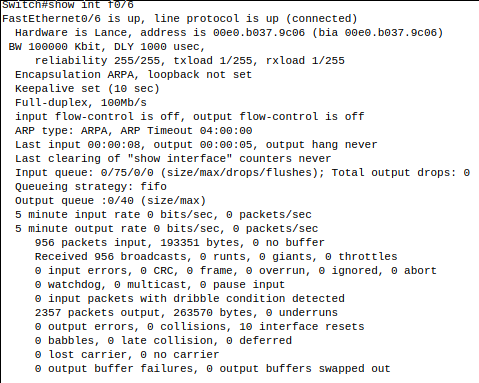
\includegraphics[width=.45\linewidth]{Figures/2020-02-20-130138_479x383_scrot.png}}\par
\subfloat[show vlan]{\label{Sconfig9showvlan}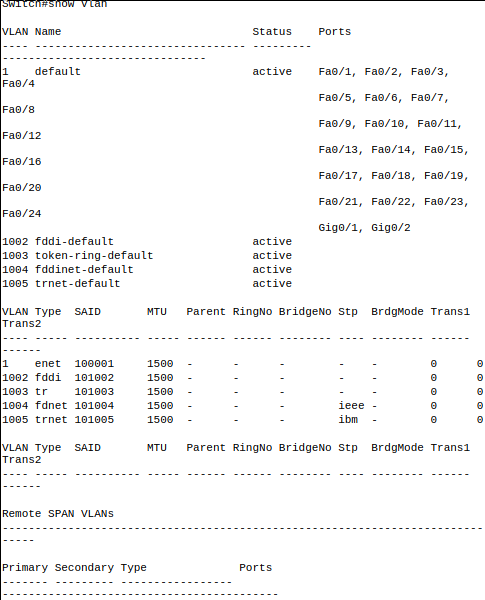
\includegraphics[width=.45\linewidth]{Figures/2020-02-20-130203_485x600_scrot.png}}\hfill
\subfloat[show flash]{\label{Sconfig9showflash}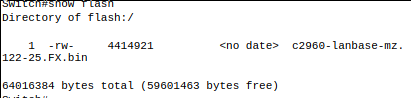
\includegraphics[width=.45\linewidth]{Figures/2020-02-20-130223_411x98_scrot.png}}\par
\caption{Configuring and Verifying the switch Pt 3}
\label{Sconfig9.3}
\end{figure}

\clearpage


%===================================
\mysection{\textbf{Part 2: Configure Basic Network Device Settings}}


\mysubsection{1}{Configure basic switch settings}
I ran pasted the commands as shown by you.I ran the commands to setup the ip 
address and default ip address. I set up the console and setup the vty. 
The login command is required because it logs in
the first time and makes us use the password afterwards.
\hfill\break

\noindent\mysubsection{2}{Configure IP address on PC-A}
\\I logged into PC-A and configured the ip configuration according to the table

%===================================
\mysection{\textbf{Part 3: Verify and Test Network Connectivity}}

\mysubsection{1}{Display the switch configuration}
You can see in Fig.~\ref{verify9}~\subref{verify9showrun} 
on Pg.~\pageref{verify9} and Fig.~\ref{verify9}\subref{verify9showint} on
Pg.~\pageref{verify9} that the bandwidth is 100,000 bytes,  its state is up and
its protocol is up.
\hfill\break

\noindent\mysubsection{2}{Test end-to-end connectivity with ping}
\\I ran ping from PC-A to PC-A as seen in
Fig.~\ref{verify9}\subref{verify9pingpca} on Pg.~\pageref{verify9}.
\\I then, Pinged S1 from PC-A, the first ping was lost due to address
resolution, as you can see in Fig.~\ref{verify9}\subref{verify9pings1} on
Pg.~\pageref{verify9}.
\hfill\break

\noindent\mysubsection{3}{Test and Verify Remote management of S1}
\\From PC-A I remotely logged into S1 via telnet. See
Fig.~\ref{verify9}\subref{verify9telnet} on Pg.~\pageref{verify9}.
\hfill\break

\noindent\mysubsection{4}{Saving the Switch Running Configuration File}
\\I saved the switches configuration file.

\begin{figure}[!b]\centering
\subfloat[show run]{\label{verify9showrun}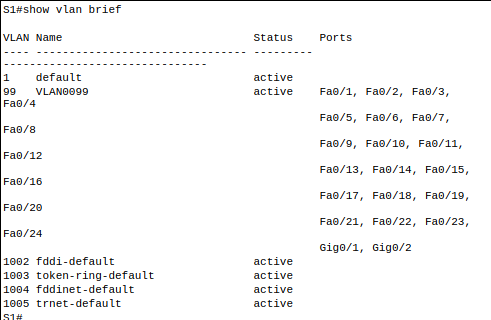
\includegraphics[width=.45\linewidth]{Figures/2020-02-20-153821_491x320_scrot.png}}\hfill
\subfloat[show interface vlan 99]{\label{verify9showint}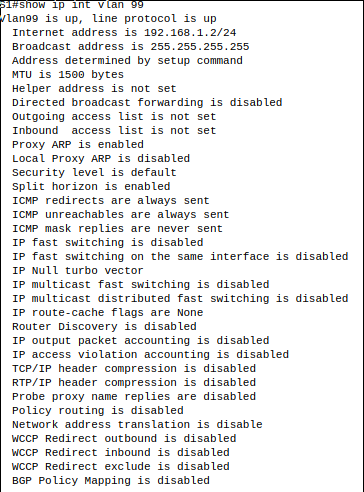
\includegraphics[width=.45\linewidth]{Figures/2020-02-20-154847_364x492_scrot.png}}\par
\subfloat[PC-A pinging PC-A]{\label{verify9pingpca}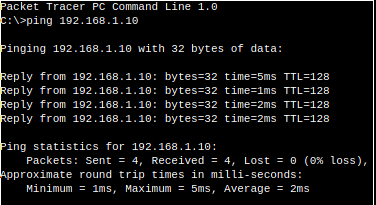
\includegraphics[width=.45\linewidth]{Figures/2020-02-20-155625_376x205_scrot.png}}\par
\subfloat[PC-A pinging S1]{\label{verify9pings1}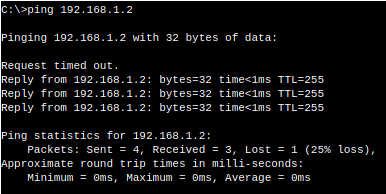
\includegraphics[width=.45\linewidth]{Figures/2020-02-20-155655_386x194_scrot.png}}\hfill
\subfloat[PC-A telnet to S1]{\label{verify9telnet}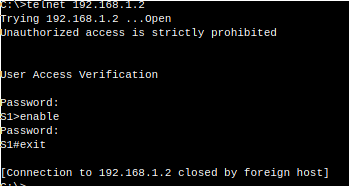
\includegraphics[width=.45\linewidth]{Figures/2020-02-20-160102_349x186_scrot.png}}\par
\caption{Verifying and Testing Network Connectivity}
\label{verify9}
\end{figure}

\clearpage


%===================================
\mysection{\textbf{Part 4: Manage the MAC Address table}}

\mysubsection{1}{Record the MAC address of the host}
\\there were none listed in the table. zero in total. 
\hfill\break

\noindent\mysubsection{2}{Determine the MAC Addresses that the switch has
learned}
\\There are three options for Mac addressing dynamic, interfaces, or static.
\hfill\break

\noindent\mysubsection{3}{List the show mac address-table options}
\\There are three options, dynamic, interfaces, or static.
\hfill\break

\noindent\mysubsection{4}{Set up a static MAC address}
\\I ran the commands as shown and set up the mac address, statically.
\hfill\break


%===================================
\mysection{\textbf{Reflection}}
\mysubsection{1}{Why should you configure the vty password for the switch?}
\\To protect it from unwanted usage where someone could set up a way into the
network and where they would have root access to the network.
\hfill\break

\noindent\mysubsection{2}{Why change the default VLAN 1 to a different VLAN
number?}
\\harder to find from cursory looks at the network.
\hfill\break

\noindent\mysubsection{3}{How can you prevent passwords from being sent in
plain text?}
\\set encryption
\hfill\break

\noindent\mysubsection{4}{Why configure a static MAC address on a port
interface?}
\\so that it stays the same and doesnt try to ask the DNS to resolve it and
risk losing it and resetting the main ports of the network.


%===================================

\end{document}
